\documentclass[../main.tex]{subfiles}

\begin{document}
In this section I will discuss the implementation details of the approach outlined in section \ref{sec:SolutionArchitecture}. Starting from the modelling of the system as Markov Decision Process, I will then describe the implementation of the Reinforcement Learning algorithm, the disturbance estimation with Gaussian Processes and finally, the safe set calculation with HJI reachability analysis.
\section{Markov Decision Process Model}\label{sec:implementation_MDP}
The dynamics of the damped inverted pendulum system are described by \cite{doya2000reinforcement}:
\begin{align}
    \dot{x_1} &= x_2\\
    \dot{x_2} &= \frac{1}{ml^2}u+\frac{g}{l}\sin(x_1)-\frac{b}{m}x_2+d(x)
\end{align}
where $m$ is the mass of the pendulum, $l$ is the length of the pendulum, $g$ is the gravity constant and $b$ is the friction coefficient. All constants can be assumed to be positive. 
Modelling the inverted pendulum system as a MDP means to define the quintuple $(S,A,T,r,\gamma)$ as defined in \ref{sec:RL}. Defining the finite set of states $S$ and the finite set of actions $A$ implies discretization over the intervals $[x_{min}, x_{max}]$ and $[u_{min}, u_{max}]$ where $x_1$ is a circular state and should be wrapped if the discretization interval is larger than its period $2\pi$. The number of discretization  steps is important for the convergence speed of the Reinforcement Learning algorithm and was chosen around $n = 20$ for each state dimension.
The transition probabilities $T$ have been approximated by simply sampling the discrete transitions under a chosen time step $h$. Given a specific action and state, the subsequent state has been simulated 100 times. The probability $P(s'|s,a)$ of state $s'$ is then computed as the number of transitions to $s'$ from the chosen state and action divided by the number of total transitions. It is important that the time step $h$ is large enough to actually allow transitions. It $h$ is too small the system will always stay in state $s$ regardless of the chosen action. For the system we consider the time step should lie around $h = 0.2$. The reward function $r(s)$ is defined as
\begin{equation}
    r(s) = e^{-\frac{||s||^2}{\sigma^2}};
\end{equation}
where $\sigma$ is a constant defining how narrow the reward function is. Defining the coordinate system with $x_1 = 0$ being on the top, this reward corresponds to the goal to keep the pendulum still and upright as the states with the smallest $x$ are rewarded the most. The discount factor $\gamma$ is chosen to be $0.9$.
\section{Reinforcement Learning}
On the obtained MDP Reinforcement Learning was then applied to learn an optimal control policy. The chosen algorithm is a slightly modified version of the in section \ref{sec:RL} introduced Delayed Q-Learning. 
\input{Chapters/algo1.tex}
In large parts the algorithm resembles the Delayed Q-Learning algorithm that was introduced in \ref{sec:RL} with the update rule \eqref{DelayedQ}. The only difference lies in the handling of the algorithm inputs $\varepsilon$ and $m$. The batch size $m$ determines how often the update of a state-action pair's Q-value is attempted until a successful update of any Q-value has to occur for the update to be attempted again. This batch size has been replaced by the state-action-dependent batch size $M(s,a)$ that is increased each time when the update of the state-action pair $(s,a)$ has been tried $M(s,a)$ times. The update rule is 
\begin{align}
    M_{t+1}(s_t,a_t) &= \min\{\lceil1.02M_t(s_t,a_t)\rceil+1, 500\}\\
    M_{t+1}(s,a) &= M_t(s,a) \qquad \forall (s,a) \neq (s_t,a_t)
\end{align}
The threshold $\varepsilon$ for an update to be admitted has been made adaptive such that $\varepsilon$ after $M(s,a)$ attempted updates increases to 
\begin{equation}
    \varepsilon_{t+1} = \min\{1.1 \varepsilon_t, \varepsilon_{\text{target}}\}.
\end{equation}
The initialization of the Q-values is done optimistically according to \eqref{eq:optimistic_init}. The learning rate is chosen to be $\alpha = \frac{1}{v+1}$ where $v$ is the number of times that the current state action pair has been visited. This learning rate leads to a faster convergence than $\alpha = \frac{1}{n+1}$ with iteration count $n$ and fulfills still the convergence criteria posed in \eqref{eq:stepsize}. Without any safety-preserving controller, this algorithm converges to the optimal policy but does not guarantee any constraint satisfaction. Figure \ref{fig:PolicyComparison_unsafe} shows the learned policy after a test run with $100000$ steps in comparison to the optimal policy that has been found with policy iteration. The colours correspond to certain action values. It can be seen that the estimated policy is relatively accurate, however the learning algorithm violates the boundaries of the MDP no less than $8986$ times. The number of constraint violations is decreasing over time as can be seen in figure \ref{fig:Histogram_ConstraintViolations} because the algorithm learns the optimal policy but safety can never be guaranteed. To prevent those violations from happening, a safe controller will be introduced in the next section.


\begin{figure}[h]
    \centering
    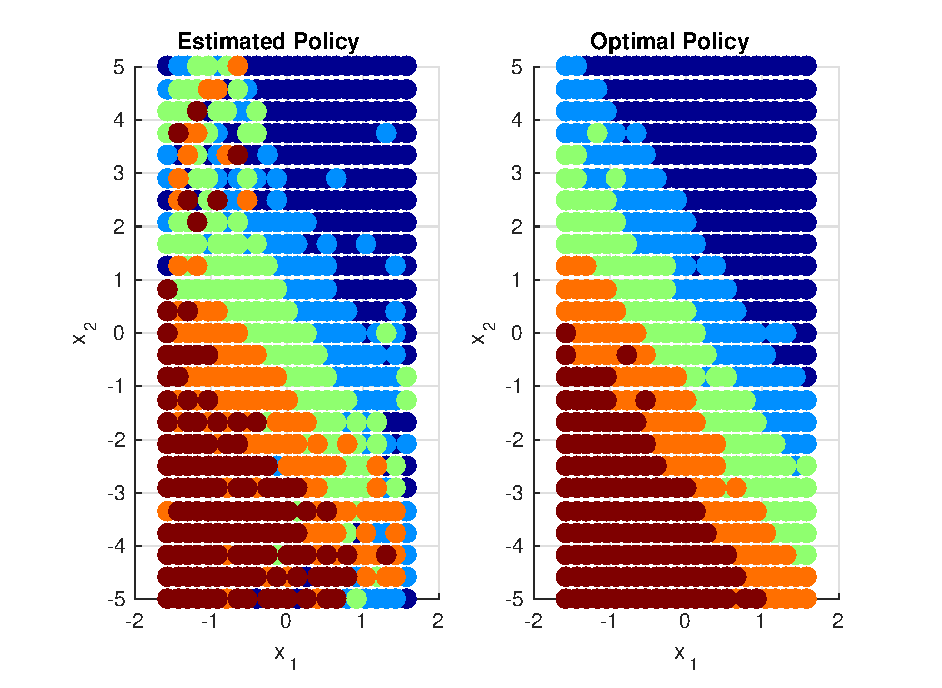
\includegraphics[width=\textwidth]{PolicyComparison_unsafe}
        \caption{Comparison between the learned policy and the with policy iteration determined optimal policy.}    
    \label{fig:PolicyComparison_unsafe}
\end{figure}
\begin{figure}[h]
    \centering
    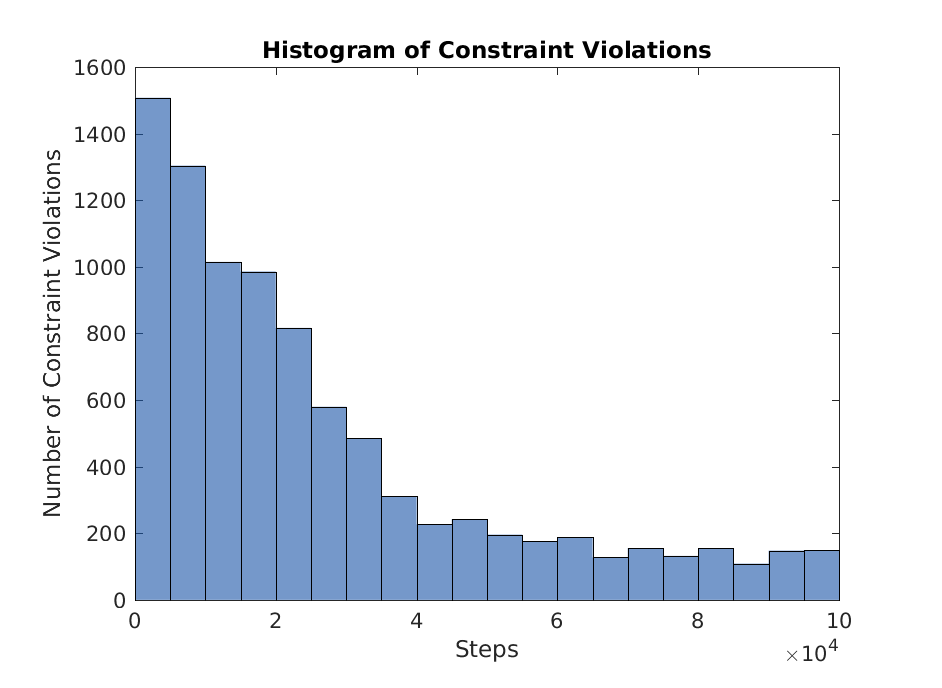
\includegraphics[width=\textwidth]{Histogram_ConstraintViolations}
        \caption{Evolution of the constraint violations over .}    
    \label{fig:Histogram_ConstraintViolations}
\end{figure}

\section{Safe Set Computations based on Reachability Analysis}
The general idea behind safe set computations has been described in chapter \ref{sec:SafeSets}. In this section the concrete implementation on the inverted pendulum system will be described. The Hamiltonian in this case becomes 
\begin{equation}\label{eq:hamil_implementation}
    H(x,p) = \max_{u \in \mathcal{U}} \min_{d \in \mathcal{D}} p^T 
\left(
\begin{array}{c}
x_2\\
\frac{1}{ml^2}u+\frac{g}{l}\sin(x_1)-\frac{b}{m}x_2+d\\
\end{array}
\right).
\end{equation}
Determining the optimizers to \eqref{eq:hamil_implementation} can be done easily for non-linear systems whose inputs enter linearly. That means that the dynamics can be written on the form
\begin{equation}
    f(x,u,d) = f^x(c)+\textbf{F}^u(x)u+\textbf{F}^d(x)d.
\end{equation}
This is the case for the inverted pendulum system with
\begin{align}
    f^x(x) &= \left(
\begin{array}{c}
x_2\\
\frac{g}{l}\sin(x_1)-\frac{b}{m}x_2\\
\end{array}
\right)\\
    \textbf{F}^u(x) &= \left(
\begin{array}{c}
0\\
\frac{1}{ml^2}\\
\end{array}
\right)\\
    \textbf{F}^d(x) &= \left(
    \begin{array}{c}
0\\
1\\
\end{array}
\right).
\end{align}
According to \cite{mitchell2004toolbox}, the input maximising \eqref{eq:hamil_implementation} and the disturbance minimizing the equation are then given by 
\begin{align}
    u^*(x,p)&=
\begin{cases}
  \underline{U},\qquad \text{if} \sum_{j=1}^n p_j \textbf{F}^u_j(x)\leq 0;\\
  \overline{U}, \qquad \text{otherwise}
\end{cases}\\
    d^*(x,p)&=
\begin{cases}
  \overline{D},\qquad \text{if} \sum_{j=1}^n p_j \textbf{F}^d_j(x)\leq 0;\\
  \underline{D}, \qquad \text{otherwise}.
\end{cases}
\end{align}
The values in the curly brackets describe the input constraints $u\in \mathcal{U} = [\underline{U},\overline{U}]$ and disturbance bounds $d\in \mathcal{D} = [\underline{D},\overline{D}]$. By defining 
\begin{align}
    U^{\text{max}} &= \max(|\underline{U}|,|\overline{U}|) \\
    D^{\text{max}} &= \max(|\underline{D}|,|\overline{D}|), 
\end{align} 
$u^*$ and $d^*$ can be explicitly written as
\begin{align}
    u^* &= \frac{1}{ml^2} U^{\text{max}} \text{sign}(p_2)\\
    d^* &= -D^{\text{max}} \text{sign}(p_2).
\end{align}
This results in the Hamiltonian
\begin{equation}\label{eq:hamil_explicit}
    H(x,p) = p_1x_2+p_2\left(\frac{g}{l}\sin(x_1)-\frac{b}{m}x_2\right)+|p_2|\left(\frac{1}{ml^2}U^{\text{max}}-D^{\text{max}}\right)
\end{equation}
that needs to be coded into an existing function prototype within the toolbox.
To calculate the derivative $p = \frac{\partial}{\partial x} \phi(x,t)$ the Level Set toolbox employs the Lax-Friedrichs approximation 
\begin{equation}
    \hat{H}(x,p^+,p^-) \overset{\Delta}{=} H\left(x,\frac{p^-+p^+}{2}\right) - \frac{1}{2} \alpha^T(p^+-p^-)
\end{equation}
where $p^+$ and $p^-$ are left and right side approximations of $p$. $H(x,p)$ is given by \eqref{eq:hamil_explicit}.  
\begin{equation}
    \alpha_i(x) = \max_{p\in\mathcal{I}} \left|\frac{\partial H}{\partial p_i}\right|
\end{equation}
with $\mathcal{I}$ being the hypercube containing all values that $p$ takes over the computational domain needs to be implemented within the provided function prototype. This can be done with the over-approximation
\begin{equation}
    \alpha_j(x) \leq |f_j^x(x)| + |\textbf{F}_j^u|U^{\text{max}} + |\textbf{F}_j^d|D^{\text{max}} 
\end{equation}
that for the present system resolves to 
\begin{align}
    \alpha_1 &\leq |x_2|\\
    \alpha_2 &\leq \left|\frac{g}{l}\sin(x_1)-\frac{b}{m}x_2\right| + \frac{1}{ml^2}U^{\text{max}} + D^{\text{max}}.
\end{align}
Having specified the functions for calculating $H(x,p)$ and $\alpha(x)$, the Level Set toolbox can be adapted for the present problem. Specifically, a function has been written that takes as inputs an estimate for the disturbance bounds $\underline{D}$ and $\overline{D}$, input constraints $\underline{U}$ and $\overline{U}$ an initial safe set $\mathcal{S}_0$, a time horizon $\tau$ and the state space of the MDP and outputs for each state in the MDP if it is safe or not under time horizon $\tau$ and a safe control $u^*$ for each state. During the learning process, one can then apply the safe control as soon as the system hits the border of the safe set. To illustrate this, figure \ref{fig:safeSet_example} shows the evolution of a safe set calculation over the time horizon $\tau = 30s$. The first subplot shows the initial safe set $\mathcal{S}_0$ as defined by the function input. Over time, the safe set is shrinking to the set $\mathcal{S}_\tau$ that is shown in the last subplot. Trajectories that start from within this set are guaranteed to remain in $\mathcal{S}_0$ for $t = [0, \tau]$. It can easily be seen that the set converges already within the first seconds such that trajectories that are safe for $t = [0, 10]$ are also safe for the whole time horizon. 

\begin{figure}[h]
    \centering
    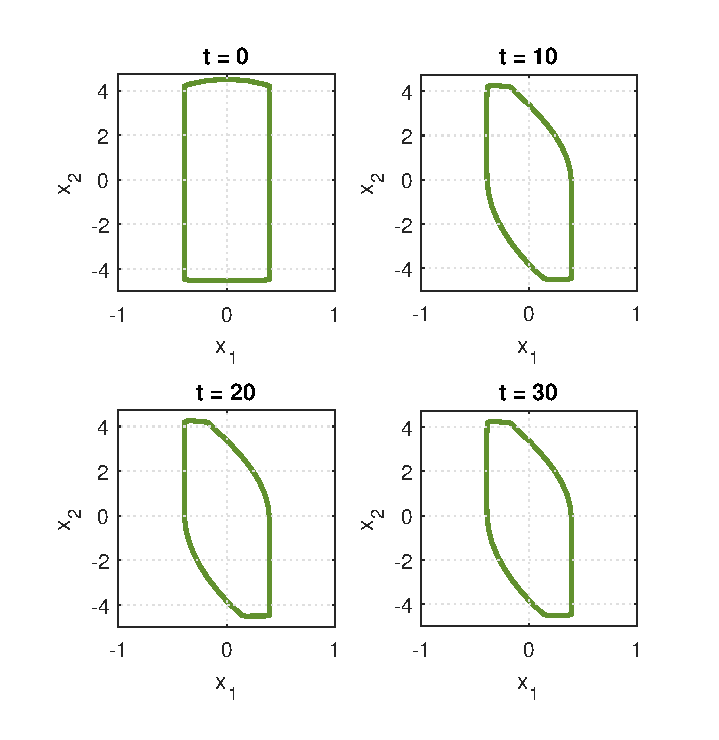
\includegraphics[width=\textwidth]{safeSet_example}
        \caption{Example for the evolution of a safe set during the time horizon.}    
    \label{fig:safeSet_example}
\end{figure}

Moreover, to verify the calculations simulations of system trajectories have been done for both, initial conditions within the safe set $\mathcal{S}_\tau$ and without that set. The results can be seen in figure \ref{fig:safeSet_simulation}. Trajectories are marked with a red dot at the initial condition and a blue dot at the final value. The safety-preserving controller manages to keep all trajectories with initial conditions inside $\mathcal{S}_\tau$ within the safe set for the complete simulation time. The simulation time has been chosen to be smaller than the time horizon $\tau$ to keep the computation time low and the figure overseeable. The result holds however also for longer simulation times. Furthermore, the figure indicates that the safe set is an under-approximation of the true safe set as also the trajectories with initial conditions close to $\mathcal{S}_\tau$ can be stabilized. Yet, no definite conclusion about that can be drawn from simulations. \par
\begin{figure}[h]
    \centering
    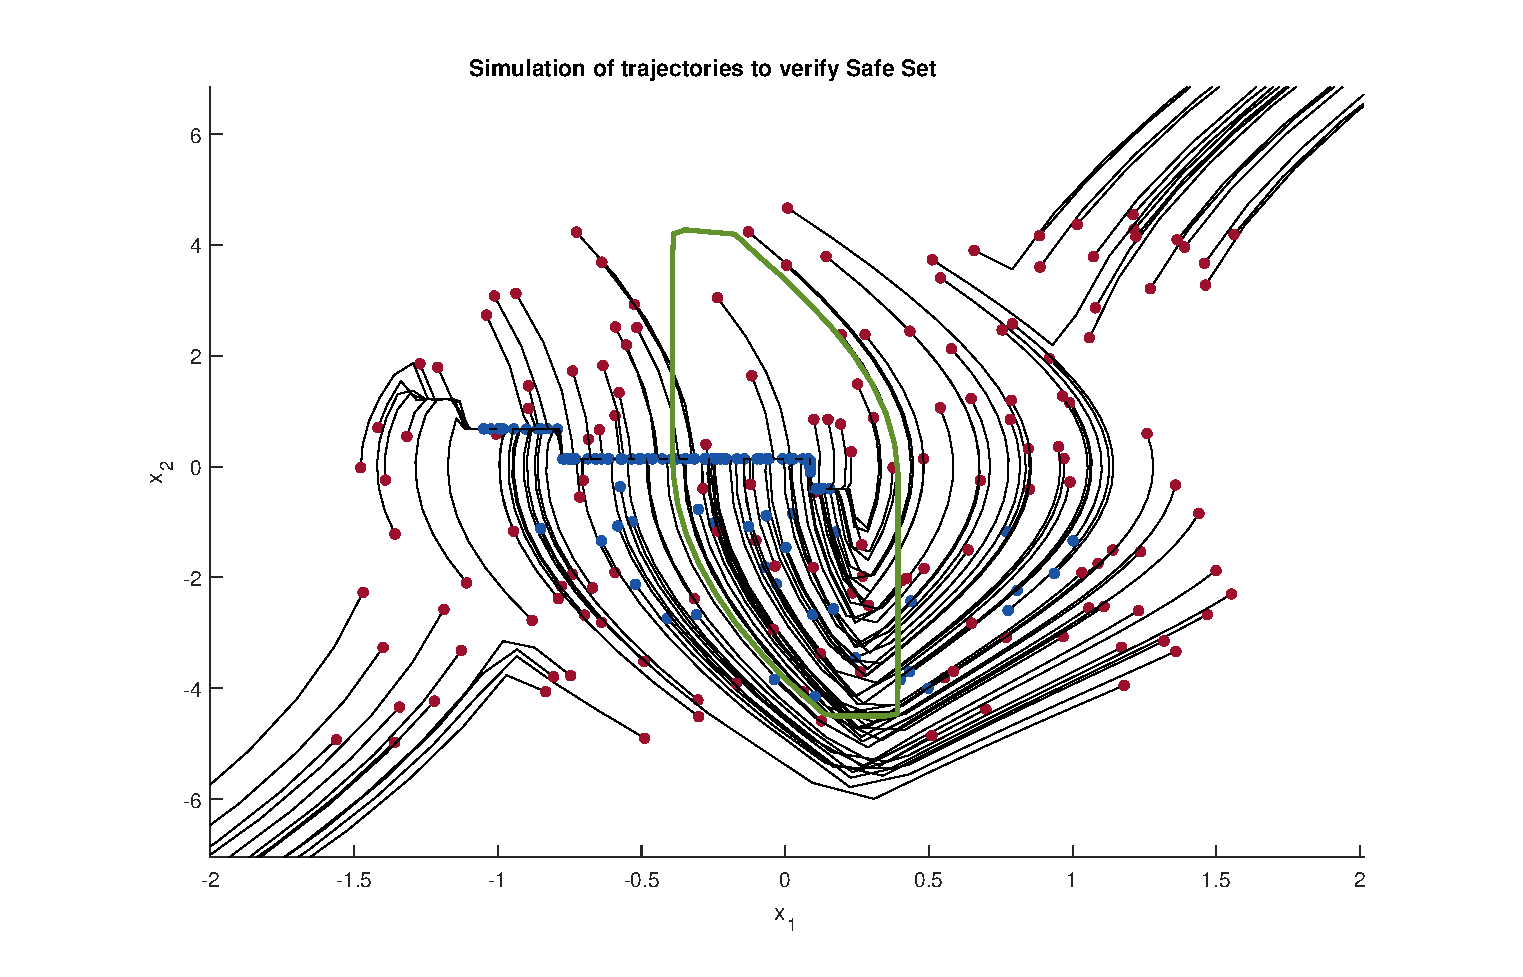
\includegraphics[width=\textwidth]{safeSet_simulation}
        \caption{Simulations to verify that all trajectories that start.}    
    \label{fig:safeSet_simulation}
\end{figure}
Another important remark is, that the safe set calculations assume continuous dynamics. It is therefore important to keep the time step $h$ small so that the error through discretization does not become too large. This conflicts with the requirement from section \ref{sec:implementation_MDP} according to which the time step should be large in order to allow transitions between states. With a very small time step learning can not take place as no state transitions can be made, a large time step can lead to instability as the system possibly violates the border of the safe set between two samples and it is then not guaranteed that the safe control can bring the system back into that borders again. Optimally, one would find a structured way to shrink the safe set dependent on the time step in order to account for the error caused by discretization. This was however not within the scope of this thesis. This problem can be solved otherwise by introducing a "safety loop" that runs faster than the actual learning loop. For instance, if the time step required from the MDP is $h_{\text{learn}} = 0.12s$ but the time step for the safety-preserving controller should be maximal $h_{\text{safe}} = 0.02s$, the safety loop will run six times faster than the learning loop. In each safety iteration the evolution of the system is simulated. If the system violates the boundaries of the safe set, the safe control is applied, otherwise the learning control (that is constant over the six safety iterations) is applied. This can be seen in figure \ref{fig:doubleloop}. During the fourth iteration, the safe controller detects a violation of the safe set boundaries and applies the safe control that brings the system back inside the boundaries. For the sake of illustration, the time steps are chosen very large in comparison to the drawn safe set. Obviously, one would not choose the time step $h_{\text{learn}}$ that large that the whole safe set can be crossed within one time step.

\begin{figure}[t!]
    \centering
    \begin{subfigure}[t]{0.45\textwidth}
        \includegraphics[width=\textwidth]{doubleloop_fail}
    \end{subfigure}%
    ~ 
    \begin{subfigure}[t]{0.55\textwidth}
        \includegraphics[width=\textwidth]{doubleloop}
        \end{subfigure}
        \caption{Illustration of the problem with a large time step $h_{\text{learn}}$. At $t= h_{\text{learn}}$ the system is without safety check (left) already far outside the safe set so that it cannot be guaranteed to be brought back again. On the right hand side, the same example is shown with a faster running safety loop. Each $h_{\text{safe}}$ a safety check is performed so that the violation of the safe set can be detected and acted against earlier}\label{fig:doubleloop}  
\end{figure}

\section{Disturbance Estimation with Gaussian Processes}\label{sec:implementation_GP}
In this section it will be explained how the disturbance estimation with Gaussian Processes works. As stated above, the safe set calculations with HJI reachability analysis rely on a given bound for the disturbance. This bound is initially picked in a conservative manner but should be updated as soon as data from the real system are available. Given data points that have been collected during the learning process, disturbance samples can be obtained by calculating:
\begin{equation}
    \hat{d}(x)=\dot{x}_2-\left(\frac{1}{ml^2}u+\frac{g}{l}\sin(x_1)-\frac{b}{m}x_2\right).
\end{equation}
As the continuous derivative $\dot{x}_2$ is not available, an approximation with the forward difference is calculated:
\begin{equation}
    \dot{x}_2 \approx \frac{x_{2_{k+1}}-x_{2_k}}{h},
\end{equation}
where $x_{2_{k+1}}$ and $x_{2_k}$ are two consecutive samples and $h$ is the sample time.
For this approximation to be accurate, it is important that the time step $h$ is small. Therefore, the samples are recorded within the faster running safety loop, so that $h$ from the above equation is given as $h = h_{\text{safe}}$.
In order to obtain estimates for $d$ for all values of $x$ and not only for the sampled values, a Gaussian Process model is employed. Gaussian Processes also have the advantage to provide not only an estimate but with the standard deviation also an uncertainty measure so that we can pick the bounds of $d(x)$ to be
\begin{align}
    \underline{d}(x) &= \mu(x)-3\sigma(x)\\
    \overline{d}(x) &= \mu(x)+3\sigma(x),
\end{align}
where $\mu(x)$ is the mean of the estimate and $\sigma(x)$ is the standard deviation. The chosen  probabilistic bounds for $\overline{d}$ and $\underline{d}$ give a confidence interval of $99.7\%$. However, one should consider that the numerical differentiation introduces an error that is not accounted for in this confidence interval. This did not pose any problems in the algorithm, because $h_{\text{safe}}$ has been picked very small anyway to ensure safety, however, it might be interesting to account for the error due to numerical differentiation and discrete time and state space in a more structured way when calculating the safe set. \par
Another important question is how to choose sample points that can be fed to the Gaussian Process regression. As the regression is computationally expensive, it is not possible to feed all recorded samples into the Gaussian Process. One should rather choose around $1000$ points that accurately reflect the whole state space. The question then is how to ensure that the sample points are evenly spread over the whole state space, so that a good estimate over the whole state space can be obtained. To achieve this, it is not enough to randomly pick samples because the samples will (as soon as a good control is learned) concentrate around the equilibrium point. Instead, a set of randomly chosen points that covers the whole state space is used as a grid. The samples from the system that lie closest to those points are chosen so that it can be ensured that the points around the equilibrium are not over-represented.  This procedure is illustrated in figure \ref{fig:pointchoice}. One should notice that all chosen samples still will lie within the safe set, as the system is required to never leave this set. However, by getting a less conservative disturbance estimate at the borders of the safe set, it is possible to subsequently increase the safe set and therefore the region where samples can be collected.

\begin{figure}
    \centering
    \includegraphics[width=\textwidth]{pointchoice}
        \caption{Choice of samples (red) by employing a grid (blue) and taking the nearest neighbours to the grid points in order to ensure that the samples cover the whole state space.}  \label{fig:pointchoice}
\end{figure}

We then have a set of evenly spread disturbance samples that can be used for Gaussian Process regression. The regression is done with the GPML toolbox \cite{Rasmussen:2010:GPM:1756006.1953029} with a zero-mean function and a squared exponential kernel as given in \eqref{eq:sqexp}.

Figure \ref{fig:GP_posterior} aims at illustrating the results from a Gaussian Process regression for a disturbance $d = 2$ after $48000$ recorded samples of which $1000$ are fed into the Gaussian Process. The figure shows the $1000$ input samples (blue) that are widely spread within the safe set. The upper and lower plane bound the $\pm 3\sigma$ confidence interval that is additionally shaded in grey. The plane ``sandwiched" in the middle between the two outer planes is the mean, i.e. the disturbance estimate that the Gaussian Process outputs. It can be seen that the estimate in the region around the origin is very accurate and the uncertainty is low.

\begin{figure}
    \centering
    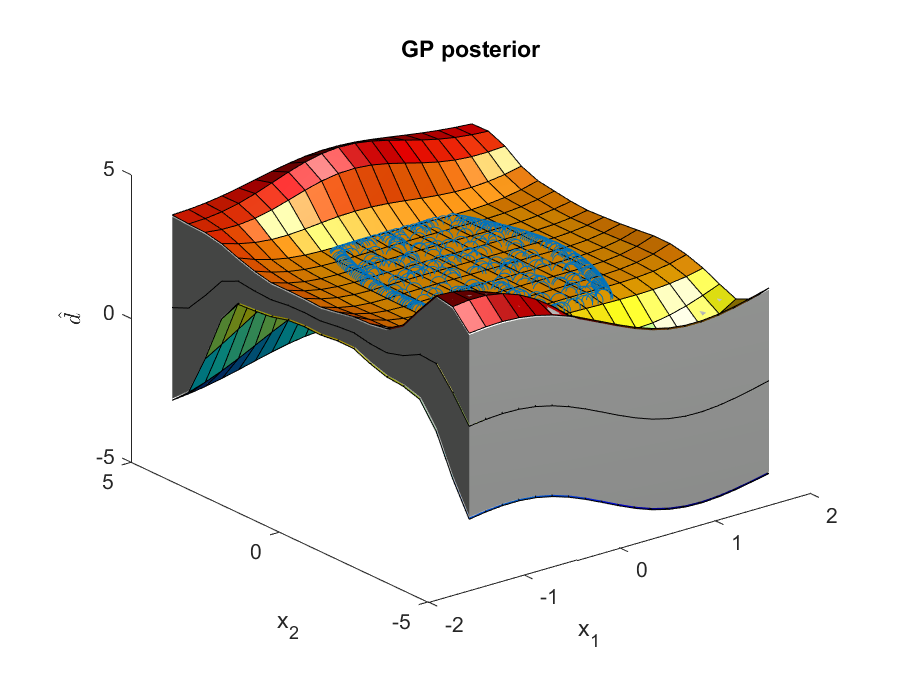
\includegraphics[width=\textwidth]{GP_posterior}
        \caption{Disturbance estimation with GP regression for a disturbance. The lower and upper plane bound the $\pm 3\sigma$ confidence interval (shaded in grey). The samples that serve as input to the GP are shown as blue circles. The mean plane can be seen as a thin line in the middle of the confidence interval.}  \label{fig:GP_posterior}
\end{figure}

\section{Exploration}
While this thesis mainly follows the approach presented in \cite{akametalu2014reachability}, this section deals with a topic that has not been treated in that approach: Exploration. Exploration describes the need of visiting the whole state space in order to find the optimal strategy instead of only exploiting already obtained knowledge of the state space. In the inverted pendulum system this describes for instance the need of also visiting the borders of the safe set in order to get a better disturbance estimate and potentially increase the safe set instead of only staying close to the origin. In section \ref{sec:implementation_GP}, the need of exploration has been dealt with in a rather unorthodox way. By setting up a grid and doing a nearest neighbour search, it has been ensured that the samples cover the whole state space. However, this is not exploration as one does not encourage the system to visit the borders of the safe set, but rather hopes for that the system does so automatically. For this reason, a more structured way of doing exploration will be presented in this section and compared to the results without exploration. The approach chosen is called incremental Q-learning and aims at a de-randomisation of the in section \ref{sec:RL} explained $\epsilon$-greedy policy \cite{even2001convergence}. Instead of choosing random actions with probability $\epsilon$, a greedy policy is chosen with respect to the $Q$-values plus a promotion term $A(s,a)$. $A(s,a)$ is initialized to zero and updated in the following way:
\begin{equation}
    A_{t+1}(s,a) = 
\begin{cases}
    0,\qquad &\text{if } s_t = s, a_t = a;\\    
    A_{t}(s,a) + \Phi_t(\#(s,a)),\qquad &\text{if } s_t = s, a_t \neq a;\\
    A_{t}(s,a),\qquad &\text{if } s_t \neq s, a_t \neq a.
\end{cases}
\end{equation}
The term $\Phi_t(\#(s,a))$ is the promotion function that depends on the number of times the system visited state $s$ without executing action $a$ since the last time it executed $a$ from $s$. The promotion function chosen in the following is $\Phi_t(i) = \frac{1}{i+1}$. This setup promotes state-action pairs that have not been visited often and therefore it encourages exploration.



\end{document}